\documentclass{article}

\usepackage{amsmath}
\usepackage{amssymb}
\usepackage{graphicx}
\usepackage{caption}
\usepackage{subcaption}
\usepackage{cite}
\usepackage{hyperref}
\usepackage{geometry}
\usepackage{fancyhdr}
\usepackage{setspace}
\usepackage{enumitem}
\usepackage{lipsum}
\usepackage{float}
\usepackage{enumitem}
\usepackage{amsfonts}

\graphicspath{ {./figures/} }



% Page layout
\geometry{top=1in, bottom=1in, left=1in, right=1in}
\pagestyle{fancy}
\fancyhf{}
\rhead{Matic Stare \and Martin Starič}
\lhead{TDA pipeline}
\cfoot{\thepage}
\renewcommand{\headrulewidth}{0.4pt}
\renewcommand{\footrulewidth}{0.4pt}

% Title
\title{TDA pipeline}

\author{
  Matic Stare
  \and
  Martin Starič
}

\date{\today}

\begin{document}

\maketitle

% Table of Contents
\tableofcontents
\newpage

\begin{abstract}
    In this report, we explore the capabilities of the TDA pipeline to classify the number of clusters within a point cloud by training a classification model. We generate synthetic data, create a filtration, build persistence diagrams and map them to an Euclidean space using persistent image vectorization. We then use statistical methods to interpret these vectors and train a classification model. Furthermore, we test our model on the Iris dataset and different synthetic data.
\end{abstract}

\section{Introduction}
The standard TDA pipeline includes creating a filtration, building persistent diagrams and mapping them to an Euclidean space using vectorization techniques, then use statistical methods to interpret the data. In this report we explore the capabilities of the TDA pipeline to classify the number of clusters within a point cloud by training a classification model.


\section{Methods}
\subsection{Synthetic training data}
To create a classification model, we require a set of data to train it on. In order to create a large enough set of data, we used an algorithm that generates a cloud of points, such that there are between $100-500$ points and $2-6$ clusters in a 3D space. We generated 1000 different instances of point clouds, where the first 200 point clouds represent data with two clusters, next 200 represent data with three clusters, and so on up to six clusters.

\begin{figure}[H]
    \centering
    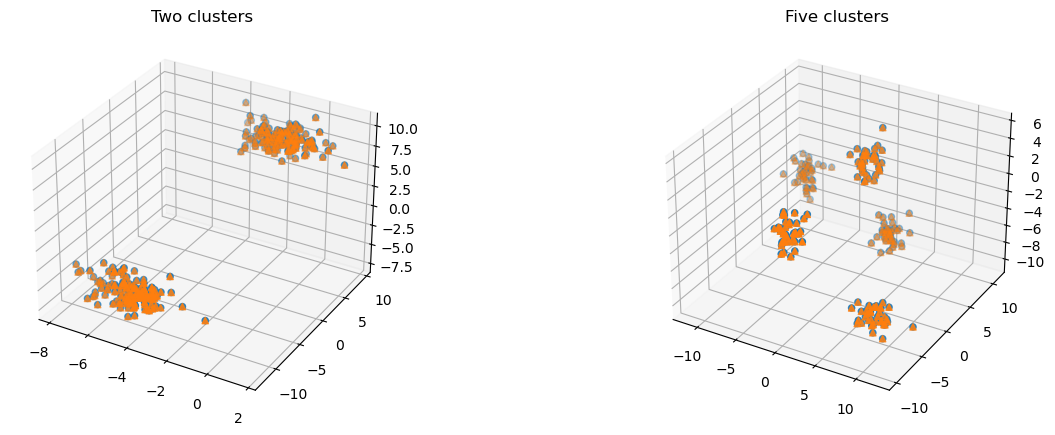
\includegraphics[width=1\linewidth]{TrainingDataViz.png}
    \caption{Training set examples, left a point cloud with two clusters, right a point cloud with 5 clusters}
\end{figure}

Above is a figure of our synthetic data, the left plot represents a point cloud that forms two clusters, while the right plot represents a point cloud that forms five clusters.


\subsection{Vietoris-Rips and Persistence diagrams}
Vietoris-Rips is our choice of filtration, due to its simplicity, which aligns with our performance goals, especially since we are only required to make persistence diagrams of dimension 0. To distinguish the number of clusters in a point cloud, we measure the number of components remaining after a certain time stamp. The majority of points would connect in the earlier parts of the filtration, whereas clusters would only connect after a much later time, that is the clusters are far enough apart. This is the reason why only dimension 0 is relevant.

\textbf{Remark} - We have attempted to use persistence diagrams with dimension 1 as well, however this captures features that actually worsen our classification model, so we decided to only use dimension 0.


\subsection{Persistent images}
To vectorize the obtained persistence diagrams, we chose persistent images. The algorithm typically creates a 2D image from each persistence diagram which we would proceed to flatten. However, since our persistence diagrams are only of dimension 0 and our birth coordinate for each component is fixed to 0, we directly obtain a one dimensional image from this vectorization. Thus, we obtain images of resolution $1 \times 100$, which is actually our output vector with 100 features. We chose the number of features to be 100, so that the algorithm would better capture when the majority of points die and when clusters start to connect.

As there is no Python implementation of persistent images for H0, we resorted to use the source code from the original authors~\cite{PIarticle} that made the algorithm in Matlab.


\subsection{Creating a classification model}
Once the persistent diagrams are vectorized, they are prepared for further analysis. The obtained vectors are first normalized, then applied to principal component analysis (PCA), a dimensionality reduction technique. With the use of PCA, the number of features in our vectors reduces enough to visually interpret and preprocess them for training purposes. The reduced vectors are then employed in training a classification model using Support Vector Machine (SVM). We chose SVM because of its robust classification capabilities and computational efficiency. To ensure that our model is not subject to overfitting, we adopted a cross-validation approach to test the accuracy of our model. We used 5-fold cross-validation, which divides our data into 5 subsets, and in each iteration, the model underwent training on four subsets and testing on the remaining one. We then compute the accuracy of each iteration to obtain the average accuracy of our model.



\section{Results}
The results of our classification model are slightly worse than expected. The accuracy on the training set is $70\%$. The model has poor accuracy when trying to classify data with 5 clusters. We can see this from figure 2, as it is evident that the classes with four, five and six clusters overlap each other. This makes that area of the graph difficult to classify for our model.

We tested our model on the Iris dataset, which does not have distinct clusters, but consists of three distinct classes (Iris setosa, Iris versicolor and Iris virginica) which is what we tried to classify. Our model classified the data incorrectly, it predicted that there were two clusters. From the graph below we can conclude that the Iris dataset is simply too different from the training set for it to be classified correctly.

\begin{figure}[H]
    \centering
    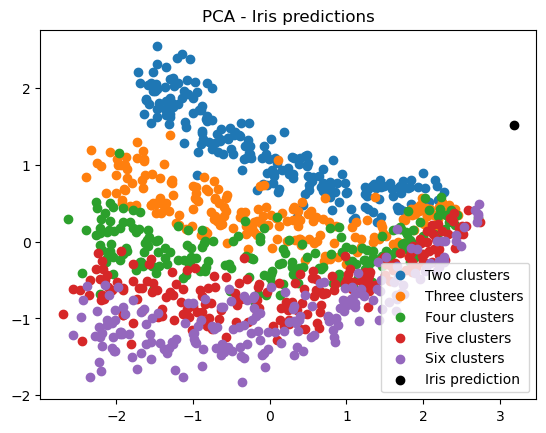
\includegraphics[width=0.49\linewidth]{PCAIris.png}
    \caption{PCA - Iris classification vector is not close enough to data, but closest to blue class}
\end{figure}

We tried to test our model on different synthetic data, this time two circles in a three-dimensional space. The two circles would represent two clusters, so our classification goal was to classify the number of clusters to be two, which ended up being the case. As seen from the graph below, the vectorized persistence diagram for the two circles data is close enough to the training set and is closest to the blue class corresponding to two clusters.

\begin{figure}[H]
    \centering
    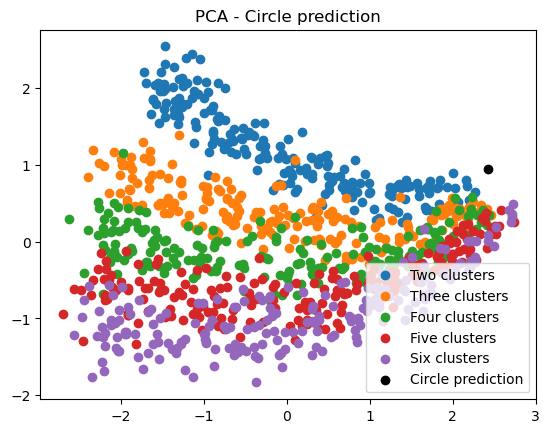
\includegraphics[width=0.5\linewidth]{PCACircles.png}
    \caption{PCA - Circles classification vector is closest to the blue class}
\end{figure}

\section{Discussion}
In this report we have explored the possibility of classifying the number of clusters in data with the help of existing topology tools. The results are not as good as we expected, perhaps this is a consequence of a poor choice of parameters in the persistent image vectorization algorithm. We observed that the persistent images we obtained, are very similar to each other. The weight function in the vectorization emphasizes the components that persist the longest. This way the points that connect within the clusters don't impact the vectorization too heavily. However, neither do the connections of clusters. This is where the problem emerges, since this is already relevant information to our classifier. We could resolve this issue by tuning parameters appropriately, however we were unable to achieve this. Another option is to take a different vectorization technique or a wider, more varied set of training data.

\section{Division of work}
Both authors worked on the entirety of the project together. We took the Extreme programming approach, where we were both working on the same code simultaneously (coding in pairs).


\bibliography{references}
\bibliographystyle{plain}
\end{document}